% !TEX TS-program = xelatex
% !TEX encoding = UTF-8 Unicode

\documentclass[11pt]{article}

% hyphenation 
\usepackage[british]{babel}

% more advanced expressions in \setlength
\usepackage{calc}

% force usage of newer commands (optinonal) 
\usepackage[l2tabu,orthodox]{nag}

% define margin
\newlength\cvMargin
\setlength\cvMargin{1cm}

\usepackage[margin=\cvMargin,noheadfoot,a4paper]{geometry}

% other lengths
\newlength\cvSideWidth
\setlength\cvSideWidth{0.3\paperwidth-\cvMargin}

\newlength\cvMainWidth
\setlength\cvMainWidth{\paperwidth-4\cvMargin-\cvSideWidth}

\newlength\cvPictureWidth
\setlength\cvPictureWidth{4cm}

\newlength\cvLanguageBarWidth
\setlength\cvLanguageBarWidth{5em}

\newlength\cvLanguageBarHeight
\setlength\cvLanguageBarHeight{0.75em}

% links
\usepackage{hyperref}

% more advanced command definitions
\usepackage{xparse}

% advanced drawing
\usepackage{tikz}
\usetikzlibrary{calc,positioning,backgrounds,matrix}

% pictures
\usepackage{graphicx}

% define four main colours
\definecolor{cvGreen}{HTML}{357F2D}
\definecolor{cvGreenLight}{HTML}{B8E4B3}
\definecolor{cvDark}{HTML}{2F3142}
\definecolor{cvAccent}{HTML}{474A65}

% load external fonts
\usepackage{fontspec}    

% icon font
\usepackage{fontawesome}   
   
% load external fonts
\setmainfont[Numbers={OldStyle,Monospaced}]{Fira Sans}
\setsansfont{Fira Sans}
\setmonofont{Fira Mono}

\pagestyle{empty}

% update default paragraph indent, and header space
\setlength{\topskip}{0pt}      % between header and text (0 needed for vertical centring)
\usepackage{parskip}           % remove paragraph indents

% set TikZ styles
\tikzset{
  contactIcon/.style={%
    minimum height=\baselineskip,
  },
  contactText/.style={%
    minimum height=\baselineskip,
    text depth=0pt,
  },
  headerIcon/.style={
    minimum width=\headericonwidth,
    anchor=center,
  },
  languageText/.style={},
  progressArea/.style={%
    draw,
    rectangle,
    minimum width=\cvLanguageBarWidth,
    minimum height=\cvLanguageBarHeight,
    cvGreen},
  progressBar/.style={%
    minimum height=\cvLanguageBarHeight,
    rectangle,
    draw,
    fill,
    cvGreen,
    anchor=west},
  }

% based on https://tex.stackexchange.com/questions/65731
\makeatletter
\def\cv@hrulefill{{\color{cvGreen}\leavevmode\leaders\hrule height 1pt\hfill\kern\z@}}

% line before and after text (some tweaking is required here)
% based on https://tex.stackexchange.com/questions/15119
\NewDocumentCommand{\ruleline}{m}{\par\noindent\raisebox{\baselineskip/4}{\makebox[\linewidth]{\cv@hrulefill\hspace{1ex}\raisebox{-\baselineskip/4}{#1}\hspace{1ex}\cv@hrulefill}}}
\makeatother

\NewDocumentEnvironment{cvSideBar}{}{%
  \vspace*{\fill}
  \begin{tikzpicture}[remember picture,overlay]
    \fill[cvGreenLight] (current page.north west) rectangle ++(\cvSideWidth+2\cvMargin,-\paperheight);
  \end{tikzpicture}
  \begin{minipage}{\cvSideWidth}
    \begin{center}
}{%
    \end{center}
  \end{minipage}
  \vspace*{\fill}
}

% update global colour
\makeatletter
\NewDocumentCommand{\globalcolor}{m}{%
  \color{#1}\global\let\default@color\current@color
}
\makeatother
\AtBeginDocument{\globalcolor{cvDark}}

\NewDocumentCommand{\cvLanguage}{mm}{%
  {\globaldefs=1\relax\pgfkeys{/cv/languages/lang\the\value{languages} = #2}}
  
  \stepcounter{languages}
}
  
\begin{document}

\begin{cvSideBar}
  
  \begin{tikzpicture}
    \node[
      circle,
      minimum size=\cvPictureWidth,
      path picture={
        \node at (path picture bounding box.center){
        
\includegraphics[width=\cvPictureWidth]{images/profile_picture}
        };
      }]
      {};
  \end{tikzpicture}

  {\LARGE
  John

  \vspace{0.1cm}

  Doe}
  
  \vspace{0.5cm}
  
  {\color{cvAccent} Profession}
  
  \vspace{0.5cm}

  \ruleline{Profile}
  
  Lorem ipsum dolor sit amet, consectetur adipiscing elit. Etiam dictum imperdiet orci, at placerat nulla sagittis id. Praesent iaculis iaculis lorem a aliquam. Nam non fringilla sapien, quis posuere lectus. Quisque ac rhoncus massa. Vestibulum blandit ullamcorper nulla at posuere. In consectetur tempor sem, in interdum mi tempus nec. Cras.
  
  \vspace{4pt}
  
  \ruleline{Contact}
  
  \vspace{4pt}
  
  \begin{tikzpicture}[every node/.style={inner sep=0pt, outer sep=0pt}]
    \matrix [
      column 1/.style={anchor=center,contactIcon},
      column 2/.style={anchor=west,align=left,contactIcon},
      column sep=5pt,
      row sep=5pt] (contact) {
      \node{\faMapMarker}; 
        & \node{Some Street 5\\B-0000 City\\Country};\\
      \node{\faEnvelope}; 
        & \node{\href{mailto:me@johndoe.com}{me@johndoe.com}};\\
      \node{\faPhone}; 
        & \node{+1 781 555 1212};\\
      \node{\faGlobe}; 
        & \node{\href{https://johndoe.com}{johndoe.com}};\\
      \node{\faGithub}; 
        & \node{\href{https://github.com/johndoe}{johndoe}};\\
      \node{\faLinkedinSquare}; 
        & \node{\href{https://www.linkedin.com/in/johndoe/}{johndoe}};\\
      \node{\faTwitter}; 
        & \node{\href{https://twitter.com/JohnDoe}{@JohnDoe}};\\
      \node{\faKey}; 
        & \node{\href{https://keybase.io/johndoe}{\texttt{AAAA BBBB 0000 5555}}};\\
  };
  \end{tikzpicture}
  
  \vspace{4pt}
  
  \ruleline{Languages}
  
  \vspace{4pt}
  
  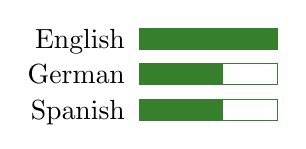
\begin{tikzpicture}[every node/.style={text depth=0pt,inner sep=0pt,outer sep=0pt}]
    \matrix [
      column 1/.style={anchor=east},
      column 2/.style={anchor=west},
      column sep=5pt,
      row sep=5pt,
      ] (contact) {
      \node[languageText]{English}; & \node[progressArea] (language 1) {}; \\
      \node[languageText]{German};  & \node[progressArea] (language 2) {}; \\
      \node[languageText]{Spanish}; & \node[progressArea] (language 3) {}; \\
    };
    \draw (language 1.west) node[progressBar,minimum width=5/5*\cvLanguageBarWidth] {};
    \draw (language 2.west) node[progressBar,minimum width=3/5*\cvLanguageBarWidth] {};
    \draw (language 3.west) node[progressBar,minimum width=3/5*\cvLanguageBarWidth] {};
  \end{tikzpicture}

\end{cvSideBar}

\end{document}